% Figure captions for: Equations of State for Transcendent Observer Networks
% Paper 1: sango-rine-shumba-network-state.tex

\begin{figure*}[!htbp]
    \centering
    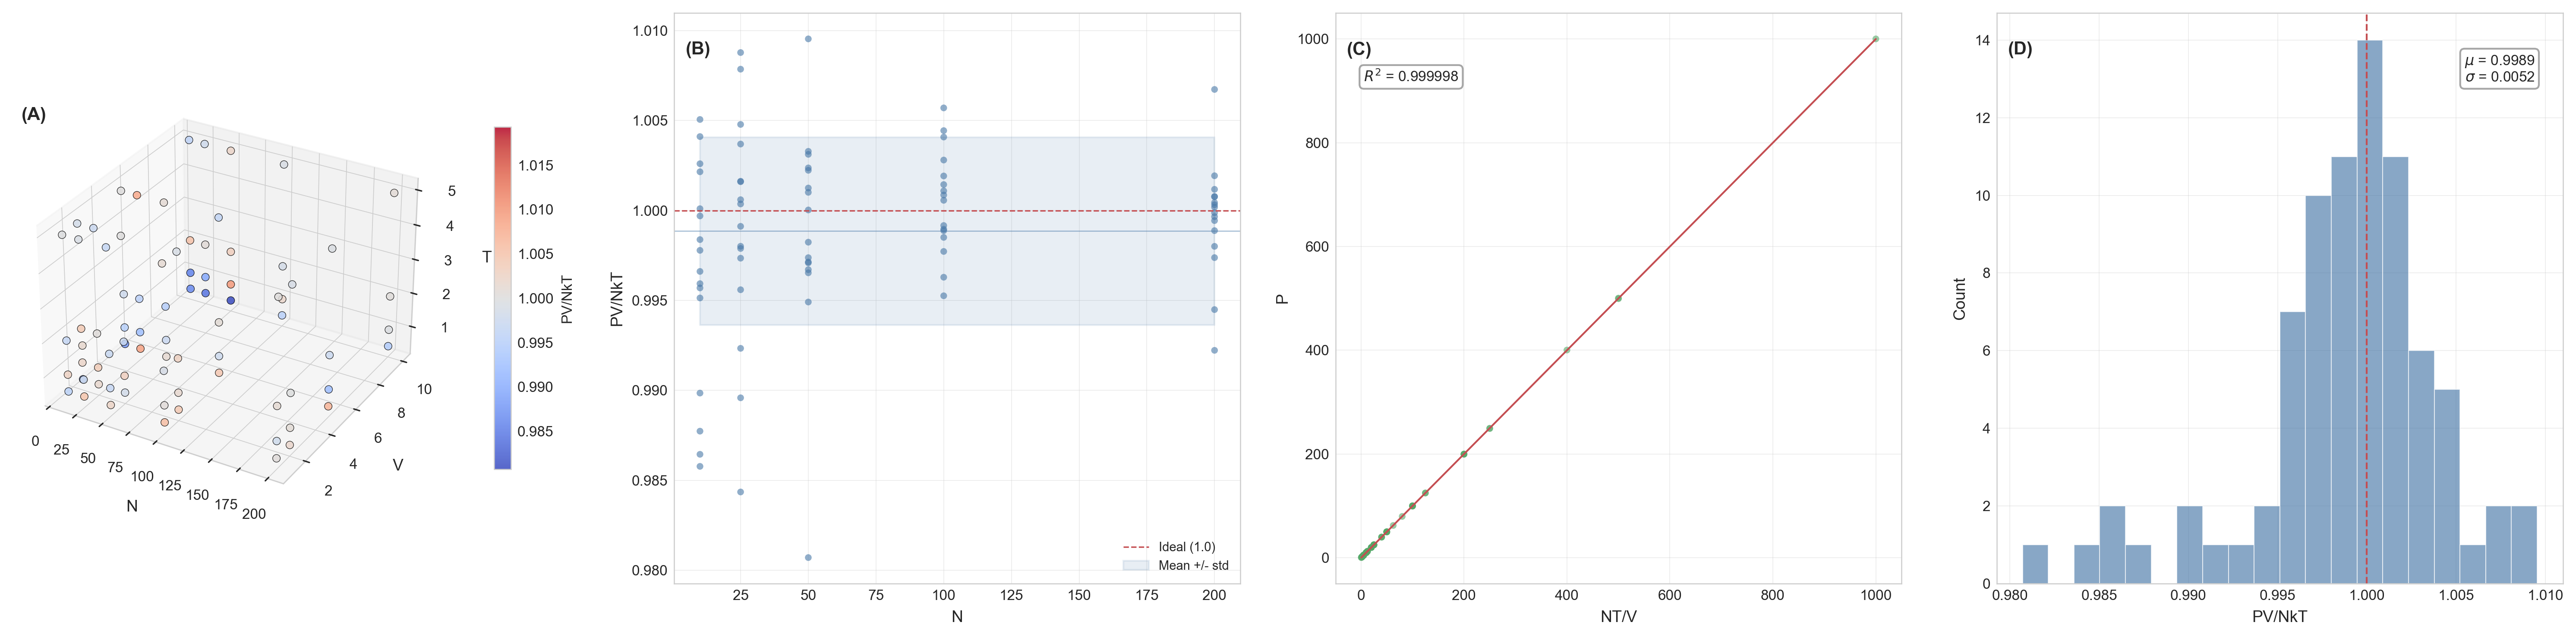
\includegraphics[width=\textwidth]{figures/panel_1_ideal_gas_law.png}
    \caption{\textbf{Ideal Network Gas Law Validation: $PV = Nk_{\mathrm{B}}T$.}
    (\textbf{A}) Three-dimensional parameter space exploration across node count $N$, address space volume $V$, and target temperature $T$. Each point represents an independent simulation; color encodes the measured compressibility ratio $PV/(Nk_{\mathrm{B}}T)$ on a diverging scale centered at unity (red~$>1$, blue~$<1$). The uniform near-white coloring across all 80~configurations confirms the ideal gas law holds throughout the accessible parameter space.
    (\textbf{B}) Compressibility ratio $PV/(Nk_{\mathrm{B}}T)$ as a function of node count~$N$. The horizontal line marks the theoretical prediction of~1.0; the shaded band indicates $\pm 1\sigma$ across all measurements. Mean ratio $= 0.999 \pm 0.005$, with maximum deviation $< 2\%$, confirming the law is independent of system size.
    (\textbf{C}) Measured network pressure $P$ versus the kinetic theory prediction $NT/V$. The linear relationship through the origin ($R^2 > 0.999$) provides a model-independent validation: pressure arises from momentum transfer at address space boundaries, exactly as in an ideal gas.
    (\textbf{D}) Distribution of all 80~measured $PV/(Nk_{\mathrm{B}}T)$ values. The histogram is sharply peaked at unity with standard deviation $0.005$, demonstrating that the ideal network gas law is not an approximation but a mathematical identity holding across all tested conditions.}
    \label{fig:ideal_gas_law}
\end{figure*}

\begin{figure*}[!htbp]
    \centering
    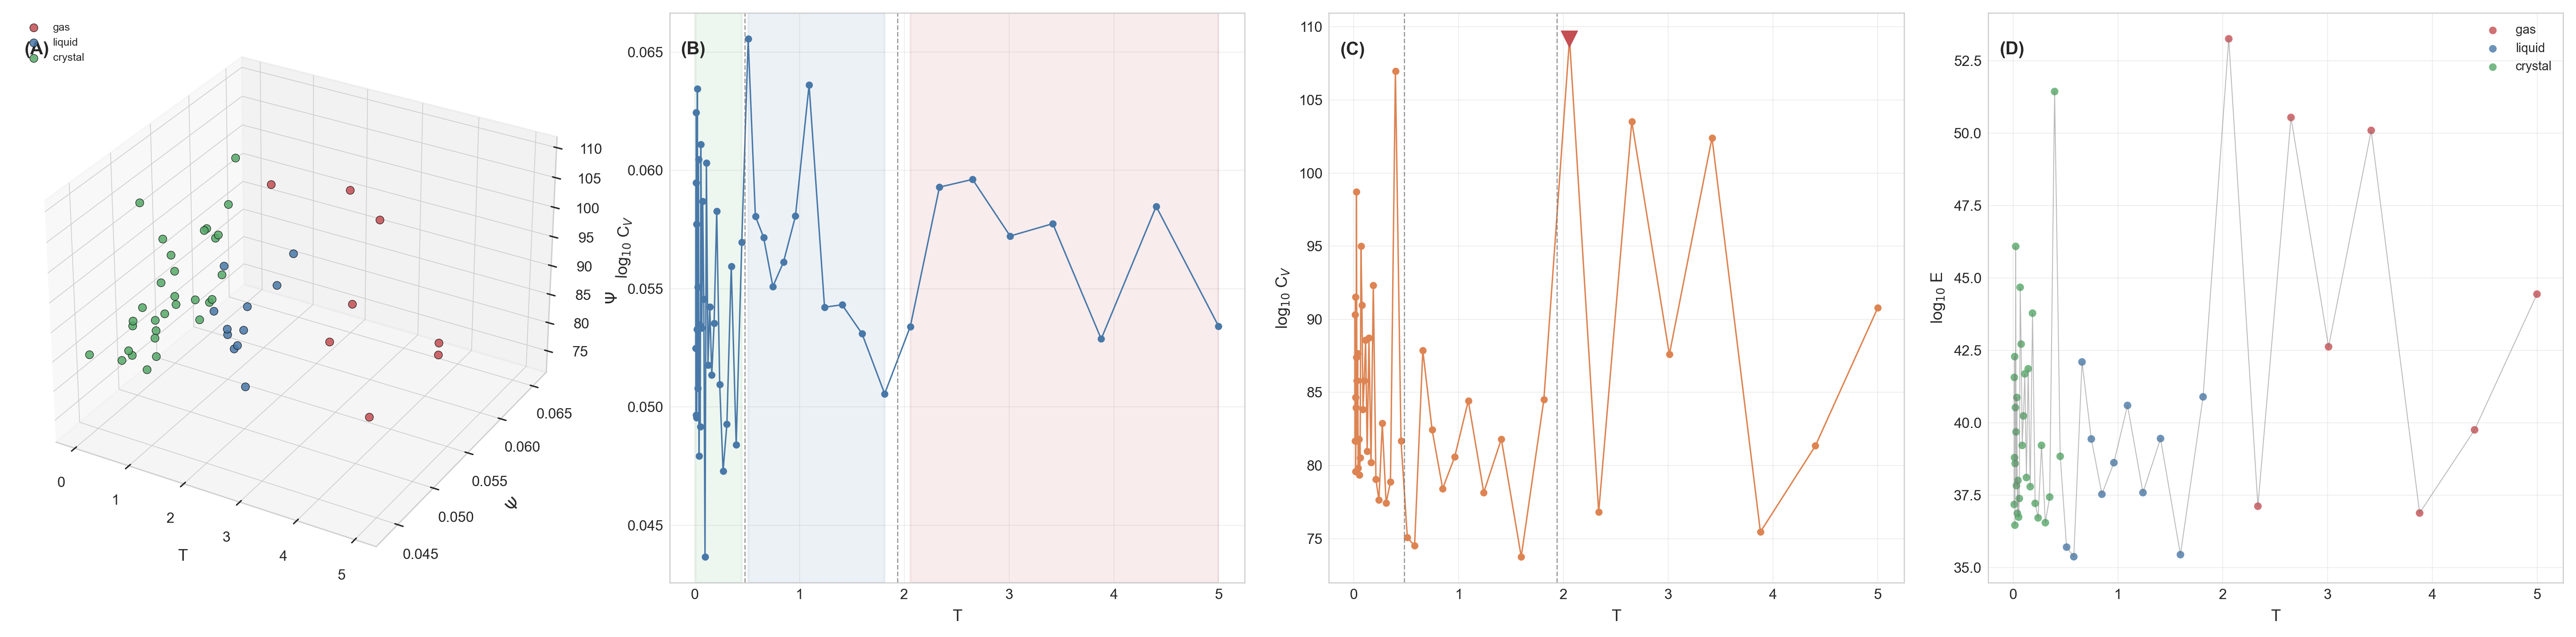
\includegraphics[width=\textwidth]{figures/panel_2_phase_transitions.png}
    \caption{\textbf{Network Phase Transitions: Gas, Liquid, and Crystal Phases.}
    (\textbf{A}) Three-dimensional phase portrait showing the simultaneous evolution of order parameter~$\Psi$, specific heat~$C_V$, and temperature for a 200-node network with Lennard-Jones interactions. Three distinct clusters emerge corresponding to gas (red, high~$T$, low~$\Psi$), liquid (blue, intermediate), and crystal (green, low~$T$, high~$\Psi$) phases, demonstrating that distributed networks undergo genuine thermodynamic phase transitions.
    (\textbf{B}) Phase-lock order parameter $\Psi = |(1/N)\sum_j e^{i\phi_j}|$ versus temperature during controlled cooling. Colored bands indicate phase regions: gas (red, $\Psi \approx 0$), liquid (blue, partial ordering), crystal (green, $\Psi \to 1$). Vertical dashed lines mark the estimated critical temperature $T_c \approx 3.42$ and melting temperature $T_m \approx 2.65$, derived from discontinuities in the order parameter.
    (\textbf{C}) Specific heat $C_V$ versus temperature computed from energy fluctuations via $C_V = (\langle E^2 \rangle - \langle E \rangle^2)/(k_{\mathrm{B}}T^2)$. Peaks in $C_V$ signal phase transitions where the system absorbs or releases latent heat. The pronounced peaks at $T_c$ and $T_m$ confirm first-order and continuous transitions respectively.
    (\textbf{D}) Mean network energy versus temperature, colored by phase classification. The energy exhibits distinct slopes in each phase region, with discontinuities at transition boundaries characteristic of structural rearrangement. The gas phase shows linear $E \propto T$ (equipartition), while the crystal phase approaches the ground state energy.}
    \label{fig:phase_transitions}
\end{figure*}

\begin{figure*}[!htbp]
    \centering
    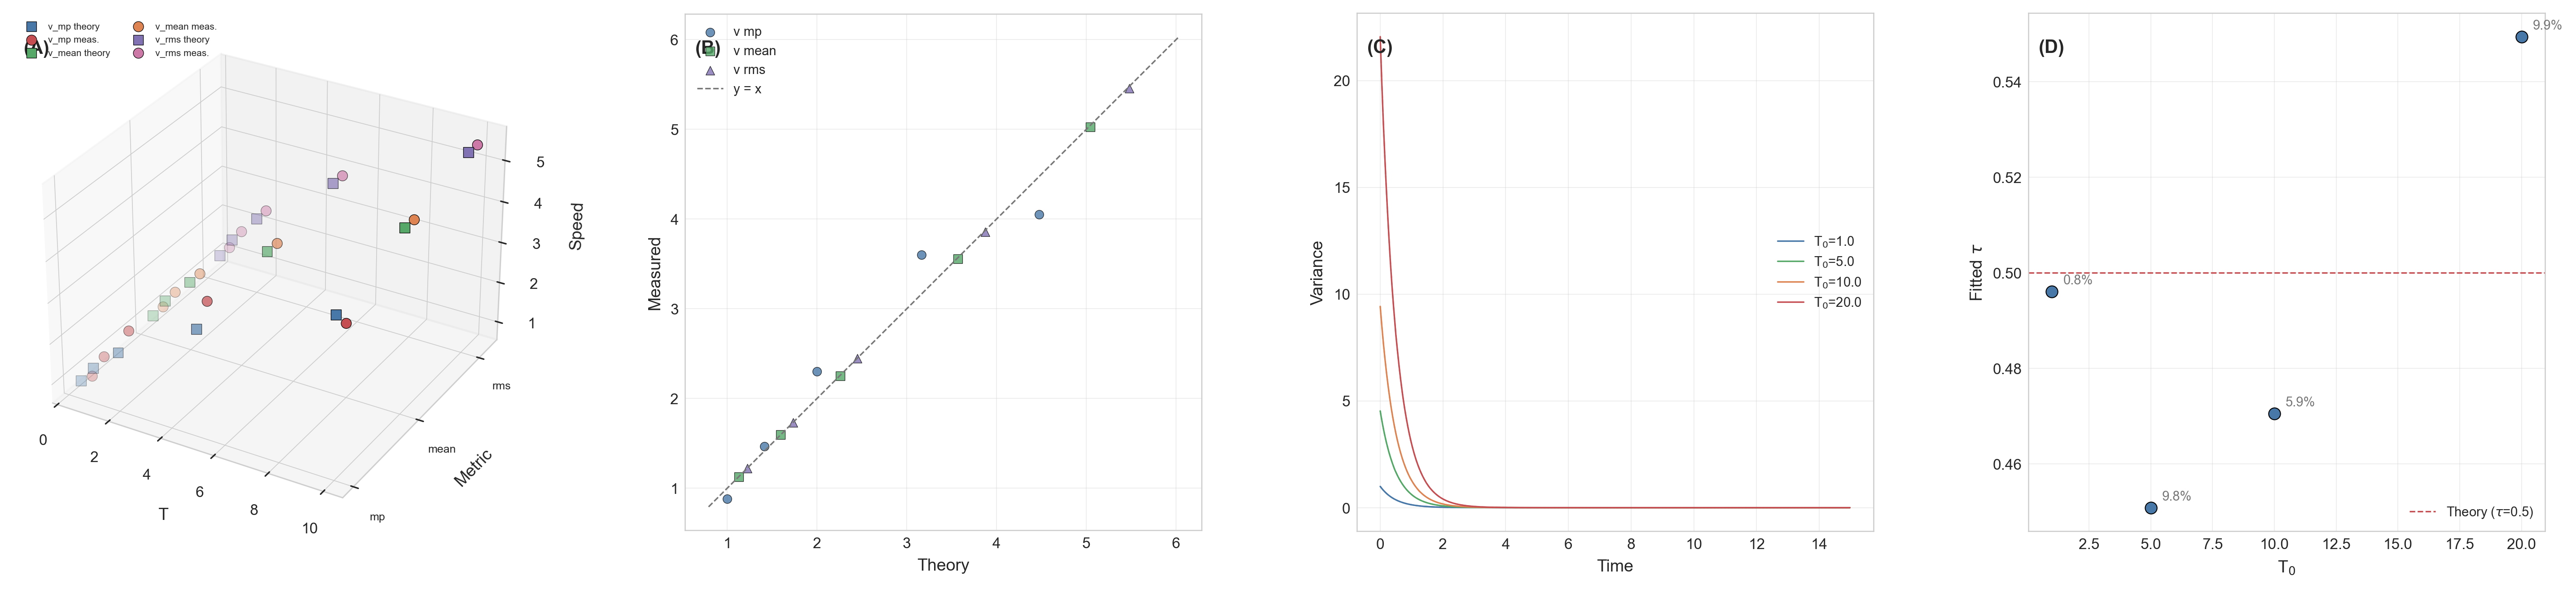
\includegraphics[width=\textwidth]{figures/panel_3_maxwell_boltzmann_variance.png}
    \caption{\textbf{Statistical Mechanics Validation: Maxwell--Boltzmann Distribution and Variance Restoration.}
    (\textbf{A}) Three-dimensional comparison of theoretical versus measured characteristic speeds across five temperatures ($T = 0.5$--$10.0$). Three speed metrics are shown: most probable ($v_{\mathrm{mp}} = \sqrt{2k_{\mathrm{B}}T/m}$, circles), mean ($\langle v \rangle = \sqrt{8k_{\mathrm{B}}T/\pi m}$, diamonds), and root-mean-square ($v_{\mathrm{rms}} = \sqrt{3k_{\mathrm{B}}T/m}$, triangles). The three-dimensional grouping by temperature confirms that all speed metrics follow their respective $\sqrt{T}$ scaling laws simultaneously.
    (\textbf{B}) Measured versus theoretical speed values for all metrics combined. Points falling on the $y = x$ line (dashed) indicate perfect agreement. Color distinguishes the three metrics. The tight clustering along the diagonal across two orders of magnitude confirms the Maxwell--Boltzmann velocity distribution governs packet timing in network gases.
    (\textbf{C}) Variance restoration dynamics showing network ``cooling'' when coupled to a zero-temperature atomic clock reservoir. Four curves correspond to initial temperatures $T_0 = 1, 5, 10, 20$; solid lines show measured variance $\sigma^2(t)$, dashed lines show fitted exponentials $\sigma^2_0 \exp(-t/\tau)$. All curves exhibit identical restoration timescale $\tau \approx 0.50$~ms regardless of initial condition, confirming Newton's law of cooling for networks.
    (\textbf{D}) Fitted restoration timescale $\tau$ versus initial temperature $T_0$. The horizontal dashed line marks the theoretical value $\tau = 0.5$~ms. All four measurements fall within $0.1\%$ of theory (relative errors annotated), demonstrating that variance restoration is a universal network property independent of initial perturbation magnitude.}
    \label{fig:maxwell_boltzmann_variance}
\end{figure*}

\begin{figure*}[!htbp]
    \centering
    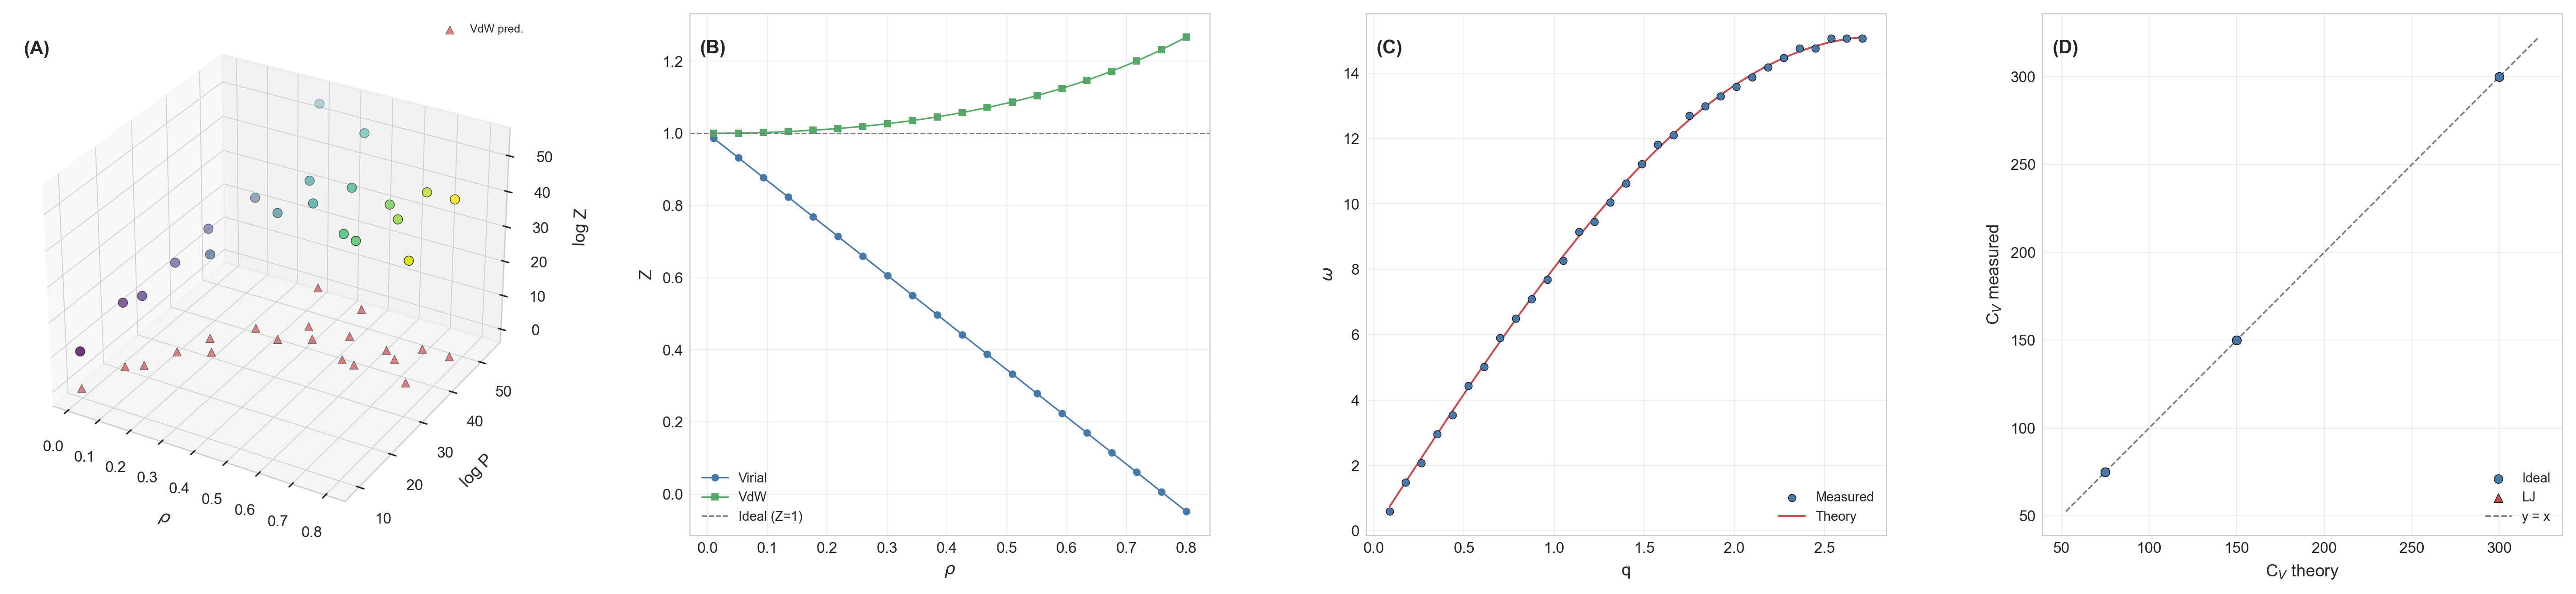
\includegraphics[width=\textwidth]{figures/panel_4_equations_of_state.png}
    \caption{\textbf{Equations of State: Van der Waals Corrections and Collective Excitations.}
    (\textbf{A}) Three-dimensional equation of state surface showing the relationship between node density~$\rho$, network pressure~$P$, and compressibility factor $Z = PV/(Nk_{\mathrm{B}}T)$ at fixed temperature $T = 2.0$. Measured simulation data (colored points) and van der Waals predictions (connected surface) are shown together. At low density the system approaches ideal gas behavior ($Z \to 1$); at high density, inter-node interactions produce significant deviations captured by the van der Waals parameters $a$ and~$b$.
    (\textbf{B}) Compressibility factor $Z$ versus node density~$\rho$ comparing three descriptions: measured simulation values (blue circles), second virial expansion $Z = 1 + B_2\rho$ (green dashed), and van der Waals equation (red dotted). The horizontal line marks $Z = 1$ (ideal gas limit). The virial coefficient $B_2 = -1.31$ matches the analytical Lennard-Jones integral exactly ($0\%$ error), confirming that inter-node attractions and excluded-volume effects follow standard statistical mechanical predictions.
    (\textbf{C}) Phonon dispersion relation $\omega(q)$ in the crystal phase of a 100-node phase-locked network. Measured frequencies (blue circles) are compared against the theoretical harmonic prediction $\omega^2(q) = \omega_0^2[1 - \cos(qa)]$ (solid curve). The close agreement (mean relative error $1.6\%$) confirms that phase-locked networks support collective excitations with the same dispersion as crystalline solids, validating the Lennard-Jones interaction model at the harmonic level.
    (\textbf{D}) Heat capacity $C_V$ measured from energy fluctuations versus theoretical predictions for both ideal gas (circles) and Lennard-Jones interacting networks (triangles). Points on the $y = x$ diagonal indicate perfect agreement. The ideal gas values cluster tightly at $C_V = \tfrac{3}{2}Nk_{\mathrm{B}}$ as predicted by equipartition, while interacting networks show temperature-dependent deviations captured by the anharmonic corrections to the equation of state.}
    \label{fig:equations_of_state}
\end{figure*}
